% Provenance (never printed): see sources/outline_sources.md (Year 1: the general
% circulation of the atmosphere, Hadley, Ferrel and polar cells, the ITCZ, Walker cells,
% jet streams, the geostrophic wind, depressions and anticyclones). Exercise and problem
% values in the Book 3 scratch calculator calc/ch28.py; figures from
% figdata/bachelor-1/angular_momentum_wind.py, weather_map.py (an invented map) and
% general_circulation.py (NCEP-NCAR Reanalysis 1, long-term means 1991-2020, datasets
% bachelor-1-ncep-{uwnd-p,vwnd-p,uwnd-sfc,slp,prate-monthly}).
% Physics owns the Coriolis force and the hydrostatic relation (recalled). Book 1 (g8) gave
% the global winds, the convection cell, depressions and anticyclones, isobars and the
% rotation of the wind around them, in words: re-founded here with forces and data.
% ENSO and the monsoons are the Year 2 volume's; the thermal wind the Year 3 volume's.
\chapter{La circulation générale de l'atmosphère}\label{ch:b1:atmospheric-circulation}

Les navires à voile qui traversaient de l'Europe et de l'Afrique vers les Amériques comptaient sur les
\omterm{def:b1:atmospheric-circulation:winds}{alizés}, vents d'est réguliers des tropiques. Plus près de l'équateur, à moins de cinq
degrés environ, les mêmes vents mouraient, dans la ceinture de calmes et d'averses persistantes
que les marins appelaient le pot-au-noir. Bien au-dessus des deux, vers neuf kilomètres
d'altitude, d'étroites rivières d'air appelées courants-jets peuvent souffler à plus de
\qty{440}{km/h}. Ce chapitre explique les trois~: pourquoi l'air en mouvement sur une planète en rotation
finit par souffler le long des isobares plutôt qu'à travers elles, comment
l'excédent des tropiques entraîne une grande cellule de retournement de chaque côté de l'équateur,
et pourquoi l'air qui quitte l'équateur en altitude se transforme en un \omterm{def:b1:atmospheric-circulation:jet}{courant-jet} d'ouest.
% ledger: nos:trade-winds, nos:doldrums, noaajs:jet

\begin{omfigure}
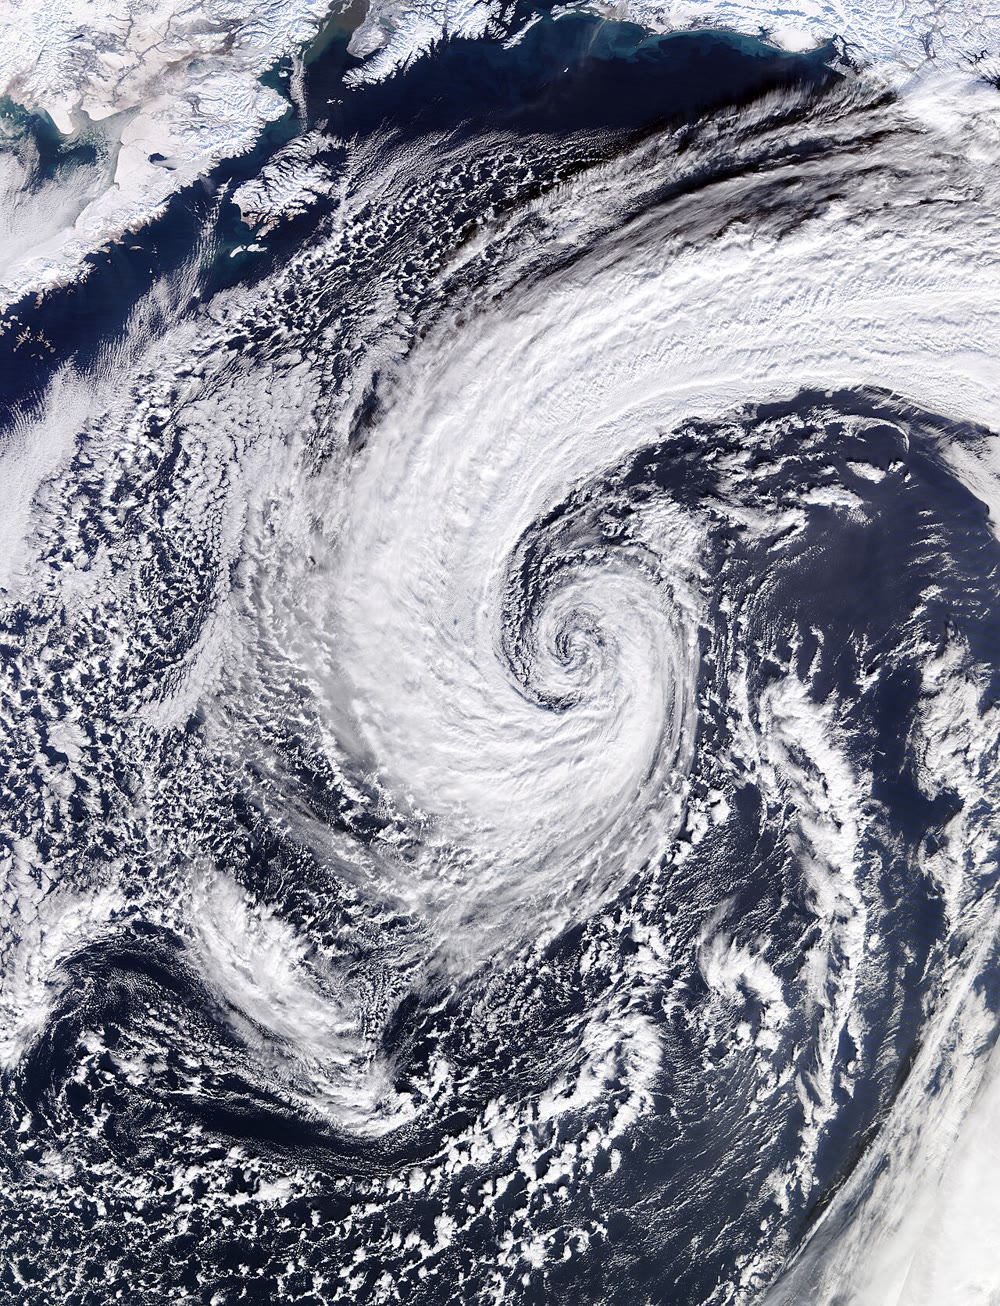
\includegraphics[width=0.5\linewidth]{images/book3/b1-alaska-low.jpg}

{\small Un \omterm{def:b1:atmospheric-circulation:cyclone}{cyclone} extratropical sur le golfe d'Alaska le 28~janvier 2018, vu
par l'instrument MODIS depuis l'orbite~; la côte enneigée de l'Alaska est en haut
à gauche, et le nord est à peu près en haut. Les bandes de nuages s'enroulent dans le sens trigonométrique vers le
centre, comme l'air d'une dépression de l'hémisphère Nord. (NASA, MODIS/LANCE,
domaine public, via Wikimedia Commons.)}
\label{fig:b1:atmospheric-circulation:alaska}
\end{omfigure}
% ledger: commons:alaska-low, nws:cyclone

\begin{recall}
Les volumes de physique donnent la relation hydrostatique et la force de Coriolis~: dans un
référentiel qui tourne à la vitesse angulaire $\vec\Omega$, un corps de masse $m$ se déplaçant
à la vitesse $\vec v$ par rapport au référentiel subit la force fictive
$-2m\,\vec\Omega\times\vec v$, perpendiculaire à son mouvement. Pour la Terre,
$\Omega = 2\pi/T_\star$ avec le jour sidéral $T_\star = \qty{23.9345}{h}$, soit
$\Omega = \qty{7.292e-5}{rad.s^{-1}}$. Le livre~1 a décrit les vents globaux (les \omterm{def:b1:atmospheric-circulation:winds}{alizés},
les \omterm{def:b1:atmospheric-circulation:winds}{vents d'ouest}, les vents d'est polaires), la cellule de convection, les dépressions et
les \omterm{def:b1:atmospheric-circulation:cyclone}{anticyclones}, les isobares d'une carte météorologique, et la rotation du vent autour des
centres. Le \cref{ch:b1:fluid-envelopes-structure} a donné l'\omterm{def:b1:fluid-envelopes-structure:standard-atmosphere}{atmosphère standard} et le
\omterm{def:b1:fluid-envelopes-structure:lapse-rate}{gradient adiabatique sec}, et le \cref{ch:b1:radiation-heat-transport} le transport de chaleur
vers les pôles que la circulation assure.
% ledger: earth:Trot, nws:coriolis
\end{recall}

\section{Les forces sur l'air en mouvement}\label{sec:b1:atmospheric-circulation:forces}

Une \omterm{def:b1:fluid-envelopes-structure:parcel}{parcelle d'air} est poussée par la pression de l'air alentour, tirée par la pesanteur,
freinée par le frottement près du sol, et, vue depuis la Terre en rotation, déviée
par la force de Coriolis. La pesanteur et la force de pression verticale s'équilibrent
presque exactement~: c'est la relation hydrostatique. Le temps est fait par les forces
qui restent dans l'horizontale.

\begin{definition}[Force de gradient de pression]\label{def:b1:atmospheric-circulation:pgf}
La \emph{force de gradient de pression}\index{force de gradient de pression} est la force nette
exercée sur une parcelle de fluide par la pression du fluide environnant. Par unité de masse elle
vaut $-(1/\rho)\nabla p$, où $\rho$ est la masse volumique et $\nabla p$ le gradient de
pression~: elle va des hautes vers les basses pressions, à travers les isobares.
\end{definition}
% ledger: nws:geostrophic

\begin{proposition}[La force de gradient de pression]\label{prop:b1:atmospheric-circulation:pgf}
Sur une parcelle de volume $\mathrm dV$ et de masse volumique $\rho$, la pression du
fluide environnant exerce la force $-\nabla p\,\mathrm dV$, soit une accélération
$-(1/\rho)\nabla p$.
\end{proposition}

\begin{proof}
Prenons une petite boîte d'arêtes $\mathrm dx$, $\mathrm dy$, $\mathrm dz$ le long des
axes. Sur sa face en $x$, la pression pousse dans la direction $+x$ avec la force
$p(x)\,\mathrm dy\,\mathrm dz$~; sur sa face en $x + \mathrm dx$, dans la direction $-x$
avec $p(x + \mathrm dx)\,\mathrm dy\,\mathrm dz$. La force nette selon
$x$ est $[p(x) - p(x + \mathrm dx)]\,\mathrm dy\,\mathrm dz = -(\partial p/\partial
x)\,\mathrm dV$, et de même selon $y$ et $z$. Le total est $-\nabla p\,
\mathrm dV$~; la division par la masse $\rho\,\mathrm dV$ donne l'accélération.
\end{proof}

Une pression uniforme n'exerce aucune force nette~: seules ses différences poussent. Sur une carte
météorologique le gradient horizontal se lit sur les isobares~: sa valeur est l'écart de pression
entre deux isobares divisé par leur distance. Pour des isobares espacées de \qty{4}{hPa} et de
\qty{400}{km} au niveau de la mer, où $\rho \approx \qty{1.225}{kg.m^{-3}}$,
l'accélération est $400/(1.225 \times \num{4e5}) = \qty{8.2e-4}{m.s^{-2}}$, moins
d'un dix-millième de $g$, et pourtant assez pour amener l'air du repos à \qty{10}{m/s} en
trois heures et demie.
% ledger: ussa76:sea-level

L'air ressent la force de Coriolis parce qu'il est observé depuis la Terre qui tourne. Sa
partie horizontale dépend de la \omterm{def:b1:spherical-astronomy:geographic}{latitude} par un seul nombre.

\begin{definition}[Paramètre de Coriolis]\label{def:b1:atmospheric-circulation:coriolis-parameter}
Le \emph{paramètre de Coriolis}\index{parametre de Coriolis@paramètre de Coriolis} à la \omterm{def:b1:spherical-astronomy:geographic}{latitude} $\varphi$ est
$f = 2\Omega\sin\varphi$, où $\Omega$ est la vitesse angulaire de la Terre. Il est
positif dans l'hémisphère Nord, négatif dans le Sud, nul à l'équateur,
et le plus grand aux pôles, $2\Omega = \qty{1.458e-4}{s^{-1}}$.
\end{definition}
% ledger: earth:Trot

\begin{proposition}[Accélération de Coriolis horizontale]\label{prop:b1:atmospheric-circulation:coriolis}
Pour un vent horizontal $\vec v$ à la \omterm{def:b1:spherical-astronomy:geographic}{latitude} $\varphi$, la partie horizontale de
l'accélération de Coriolis est $-f\,\vec k\times\vec v$, où $\vec k$ est la verticale
ascendante~: elle a pour valeur $|f|\,|\vec v|$ et est perpendiculaire au vent,
à sa droite dans l'hémisphère Nord et à sa gauche dans le Sud.
\end{proposition}

\begin{proof}
Utilisons des axes locaux $x$ vers l'est, $y$ vers le nord, $z$ vers le haut. Le vecteur rotation de la Terre est dans le
plan méridien, à l'angle $\varphi$ au-dessus de l'horizon nord~: $\vec\Omega =
\Omega(0, \cos\varphi, \sin\varphi)$. Pour $\vec v = (u, v, 0)$,
\[
  \vec\Omega\times\vec v = \Omega\,(-v\sin\varphi,\ u\sin\varphi,\ -u\cos\varphi),
  \qquad -2\vec\Omega\times\vec v = (f v,\ -f u,\ 2\Omega u\cos\varphi).
\]
Comme $\vec k\times\vec v = (-v, u, 0)$, la partie horizontale $(fv, -fu)$ est
$-f\,\vec k\times\vec v$. Le vecteur $\vec k\times\vec v$ est $\vec v$ tourné de
\ang{90} dans le sens trigonométrique vu d'en haut~; son opposé est $\vec v$ tourné dans le sens horaire,
vers la droite, quand $f > 0$, et vers la gauche quand $f < 0$.
\end{proof}
% ledger: earth:Trot

La partie verticale, $2\Omega u\cos\varphi$, vaut au plus \qty{1.5e-3}{m.s^{-2}} pour un
vent de \qty{10}{m/s}, environ \num{1.5e-4} de $g$~: l'équilibre hydrostatique
l'absorbe. La partie horizontale, si petite soit-elle, n'a pas de rivale dans l'atmosphère
libre au-dessus de la couche de frottement, et sur des heures elle façonne tout vent.

Près du sol, l'air frotte aussi contre la surface. Dans le premier kilomètre, la
couche de frottement des météorologues, le frottement change à la fois la vitesse et la
direction du vent~; des tourbillons turbulents portent vers le haut la traînée de la surface, et la
force agit à peu près contre le vent et croît avec lui. Au-dessus, dans l'atmosphère libre,
le frottement est faible.
% ledger: nws:friction-layer

\section{Le vent géostrophique}\label{sec:b1:atmospheric-circulation:geostrophic}

\begin{definition}[Équilibre géostrophique, vent géostrophique]\label{def:b1:atmospheric-circulation:geostrophic}
Un écoulement horizontal est en \emph{équilibre géostrophique}\index{equilibre geostrophique@équilibre géostrophique} quand
sa \omterm{def:b1:atmospheric-circulation:pgf}{force de gradient de pression} et sa force de Coriolis se compensent. Le \emph{vent
géostrophique}\index{vent geostrophique@vent géostrophique} $\vec v_g$ est le vent qui réalise cet équilibre pour un
champ de pression donné~: $-(1/\rho)\nabla p - f\,\vec k\times\vec v_g = \vec 0$.
\end{definition}
% ledger: nws:geostrophic

\begin{theorem}[Le vent géostrophique]\label{thm:b1:atmospheric-circulation:geostrophic}
Loin de l'équateur,
\[
  \vec v_g = \frac{1}{\rho f}\,\vec k\times\nabla p, \qquad
  |\vec v_g| = \frac{|\nabla p|}{\rho\,|f|} .
\]
Le \omterm{def:b1:atmospheric-circulation:geostrophic}{vent géostrophique} souffle le long des isobares, plus vite là où elles sont plus rapprochées.
Dans l'hémisphère Nord il garde la basse pression à sa gauche~; dans l'hémisphère
Sud, à sa droite.
\end{theorem}

\begin{proof}
Pour un vecteur horizontal $\vec w$, $\vec k\times(\vec k\times\vec w) = -\vec w$.
L'application de $\vec k\times$ à l'équilibre $f\,\vec k\times\vec v_g = -(1/\rho)\nabla p$
donne $-f\vec v_g = -(1/\rho)\,\vec k\times\nabla p$, d'où la formule, valable là où
$f \neq 0$. Comme $\vec k\times\nabla p$ est perpendiculaire à $\nabla p$, le vent est
perpendiculaire au gradient, c'est-à-dire le long des isobares~; sa valeur est $|\nabla
p|/(\rho|f|)$. Le vecteur $\vec k\times\nabla p$ est le gradient tourné de \ang{90}
dans le sens trigonométrique. En regardant dans sa direction, le gradient, qui pointe vers les hautes pressions,
est à droite, donc la basse pression est à gauche~; pour $f > 0$ le vent a
la direction de $\vec k\times\nabla p$, pour $f < 0$ la direction opposée.
\end{proof}

\begin{example}[Un vent lu sur les isobares]\label{ex:b1:atmospheric-circulation:geostrophic}
À \ang{50}~N, $f = 2 \times \num{7.292e-5} \times \sin\ang{50} = \qty{1.117e-4}{s^{-1}}$.
Des isobares espacées de \qty{4}{hPa} et de \qty{400}{km} donnent $|\nabla p| = 400/\num{4e5} =
\qty{1.0e-3}{Pa.m^{-1}}$ et, avec $\rho = \qty{1.225}{kg.m^{-3}}$, un \omterm{def:b1:atmospheric-circulation:geostrophic}{vent
géostrophique} de $\num{1.0e-3}/(1.225 \times \num{1.117e-4}) = \qty{7.3}{m/s}$. Le même
espacement à \ang{20}~N, où $f$ est moins de moitié aussi grand, donnerait
\qty{16.4}{m/s}.
\end{example}
% ledger: earth:Trot, ussa76:sea-level

L'équilibre n'est pas instantané. De l'air mis en mouvement par un gradient de pression tourne
sous la force de Coriolis au rythme $f$, environ une fois toutes les $2\pi/f$, quelque seize
heures à \ang{50}~; les configurations qui durent plus de quelques heures, et sont plus grandes que quelques
centaines de kilomètres, sont proches de l'\omterm{def:b1:atmospheric-circulation:geostrophic}{équilibre géostrophique}. Près de l'équateur $f$ tend vers
zéro, la formule cesse de valoir, et les vents des tropiques profonds ne sont pas
géostrophiques.

\begin{omfigure}
\begin{tikzpicture}[>={Stealth[length=2.2mm]}, font=\scriptsize]
  % left panel: geostrophic balance
  \begin{scope}
    \draw[isobar] (-2.4,1.2) -- (2.4,1.2) node[right] {\qty{996}{hPa}};
    \draw[isobar] (-2.4,0) -- (2.4,0) node[right] {\qty{1000}{hPa}};
    \draw[isobar] (-2.4,-1.2) -- (2.4,-1.2) node[right] {\qty{1004}{hPa}};
    \node[pressure low] at (0,2.0) {D};
    \node[pressure high] at (0,-2.0) {A};
    \fill (0,0) circle (1.6pt);
    \draw[->, very thick, omThm] (0,0) -- (0,1.0);
    \node[omThm, anchor=east] at (-0.08,0.6) {gradient de pression};
    \draw[->, very thick, omDef] (0,0) -- (0,-1.0);
    \node[omDef, anchor=east] at (-0.08,-0.6) {Coriolis};
    \draw[->, line width=1.6pt, black] (0,0) -- (1.9,0) node[above, pos=0.75] {vent $\vec v_g$};
    \node[anchor=north] at (0,-2.4) {sans frottement~: géostrophique};
  \end{scope}
  % right panel: with friction (alpha = 25 deg, V = Vg cos alpha)
  \begin{scope}[xshift=7.4cm]
    \draw[isobar] (-2.4,1.2) -- (2.4,1.2) node[right] {\qty{996}{hPa}};
    \draw[isobar] (-2.4,0) -- (2.4,0) node[right] {\qty{1000}{hPa}};
    \draw[isobar] (-2.4,-1.2) -- (2.4,-1.2) node[right] {\qty{1004}{hPa}};
    \node[pressure low] at (0,2.0) {D};
    \node[pressure high] at (0,-2.0) {A};
    \fill (0,0) circle (1.6pt);
    \draw[->, very thick, omThm] (0,0) -- (0,1.0);
    \node[omThm, anchor=east] at (-0.08,0.6) {gradient de pression};
    \draw[->, very thick, omDef] (0,0) -- ({1.0*cos(25)*sin(25)},{-1.0*cos(25)*cos(25)});
    \node[omDef, anchor=west] at (0.42,-0.62) {Coriolis};
    \draw[->, very thick, omMeth] (0,0) -- ({-1.0*sin(25)*cos(25)},{-1.0*sin(25)*sin(25)})
      node[below left, inner sep=1pt] {frottement};
    \draw[->, line width=1.6pt, black] (0,0) -- ({1.9*cos(25)*cos(25)},{1.9*cos(25)*sin(25)})
      node[above, inner sep=2pt] {vent $\vec v$};
    \draw[black!50, dashed] (0,0) -- (1.9,0);
    \draw[black!60] (1.0,0) arc[start angle=0, end angle=25, radius=1.0];
    \node[black!70] at (1.22,0.22) {$\alpha$};
    \node[anchor=north] at (0,-2.4) {avec frottement~: plus lent, à travers les isobares};
  \end{scope}
\end{tikzpicture}

{\small Forces sur une \omterm{def:b1:fluid-envelopes-structure:parcel}{parcelle d'air} dans l'hémisphère Nord, la basse pression étant au
nord. À gauche~: dans l'atmosphère libre la \omterm{def:b1:atmospheric-circulation:pgf}{force de gradient de pression} (rouge) et la
force de Coriolis (bleue) se compensent, et le vent souffle le long des isobares avec la basse à
sa gauche. À droite~: près du sol le frottement (vert) agit contre le vent~; les
trois forces ne s'équilibrent que si le vent est plus lent et dévié d'un angle $\alpha$
vers la basse (dessiné pour $\alpha = \ang{25}$ et la traînée de la
\cref{prop:b1:atmospheric-circulation:friction}).}
\label{fig:b1:atmospheric-circulation:balance}
\end{omfigure}

\begin{proposition}[Le frottement tourne le vent vers les basses pressions]\label{prop:b1:atmospheric-circulation:friction}
Supposons qu'un vent horizontal permanent $\vec v$ subisse la \omterm{def:b1:atmospheric-circulation:pgf}{force de gradient de pression},
la force de Coriolis et une force de frottement $-\vec v/\tau$, avec $\tau > 0$, à une
\omterm{def:b1:spherical-astronomy:geographic}{latitude} où $f > 0$. Alors le vent coupe les isobares vers les basses pressions à
l'angle $\alpha$ avec $\tan\alpha = 1/(f\tau)$, et sa vitesse est $|\vec v| =
|\vec v_g|\cos\alpha$, inférieure à celle du \omterm{def:b1:atmospheric-circulation:geostrophic}{vent géostrophique}.
\end{proposition}

\begin{proof}
Soit $V = |\vec v|$, $\hat v$ le vecteur unitaire le long du vent et $\hat n$ le vecteur
unitaire perpendiculaire à lui, à sa gauche. L'équilibre est $-(1/\rho)\nabla p - f\,
\vec k\times\vec v - \vec v/\tau = \vec 0$, et $\vec k\times\vec v = V\hat n$.
Le long de $\hat v$~: $-(1/\rho)\,\nabla p\cdot\hat v = V/\tau > 0$, donc le vent a
une composante descendant le gradient de pression, vers les basses pressions. Le long de $\hat n$~:
$-(1/\rho)\,\nabla p\cdot\hat n = fV$. La \omterm{def:b1:atmospheric-circulation:pgf}{force de gradient de pression}, de valeur $P =
|\nabla p|/\rho = f|\vec v_g|$, a donc pour composantes $V/\tau$ le long du vent et
$fV$ à travers lui~: elle fait avec le vent l'angle $\beta$ avec $\tan\beta =
1/(f\tau)$, et $P^2 = V^2(f^2 + 1/\tau^2)$. Les isobares sont perpendiculaires au
gradient, donc le vent les coupe sous l'angle $\alpha = \beta$, et $V = P/\sqrt{f^2 +
1/\tau^2} = (P/f)\cos\alpha = |\vec v_g|\cos\alpha$.
\end{proof}

Une surface plus rugueuse signifie une traînée plus forte, un $\tau$ plus court et un angle plus grand~:
le vent coupe les isobares plus fortement sur terre que sur mer. Le frottement réel
n'est pas exactement linéaire en fonction du vent, mais la conclusion, plus lent et dévié vers
la basse, est générale.

\begin{remark}[Le vent de gradient]\label{rem:b1:atmospheric-circulation:gradient}
Autour d'un centre les isobares sont courbes, et l'air qui les suit est accéléré
vers le centre de courbure, $V^2/r$ pour un cercle de rayon $r$. Autour d'une basse dans
l'hémisphère Nord, la \omterm{def:b1:atmospheric-circulation:pgf}{force de gradient de pression} doit alors dépasser la force de
Coriolis~: $fV + V^2/r = f|\vec v_g|$, et le vent, dit vent de gradient, est
plus faible que le géostrophique. Autour d'une haute, la force de Coriolis doit dépasser la
\omterm{def:b1:atmospheric-circulation:pgf}{force de gradient de pression}, $fV - V^2/r = f|\vec v_g|$~: le vent est plus fort, mais
l'équation n'a de solution que si $|\vec v_g| \leq fr/4$, ce qui interdit les forts gradients
de pression près du centre d'un \omterm{def:b1:atmospheric-circulation:cyclone}{anticyclone} (\cref{exo:b1:atmospheric-circulation:10}).
\end{remark}

\section{Dépressions et anticyclones}\label{sec:b1:atmospheric-circulation:cyclones}

\begin{definition}[Cyclone, anticyclone]\label{def:b1:atmospheric-circulation:cyclone}
Un \emph{cyclone}\index{cyclone} est une circulation de vents à grande échelle autour d'un centre
de basse pression, une dépression~; un \emph{anticyclone}\index{anticyclone} est une
circulation autour d'un centre de haute pression. Un cyclone tourne dans le sens trigonométrique dans
l'hémisphère Nord et dans le sens horaire dans le Sud~; un anticyclone dans le sens inverse.
\end{definition}
% ledger: nws:cyclone

Les sens de rotation découlent du \cref{thm:b1:atmospheric-circulation:geostrophic}~:
dans l'hémisphère Nord, un vent qui garde la basse à sa gauche tourne autour de la basse
dans le sens trigonométrique et autour d'une haute dans le sens horaire. Vus de l'espace, les nuages d'une
dépression dessinent la rotation (la photographie en tête du chapitre)~; dans
l'hémisphère Sud les spirales sont des images en miroir.
% ledger: nws:cyclone, commons:alaska-low

\begin{history}[La loi de Buys Ballot, 1857]
En 1857 le météorologue néerlandais C.~H.~D. Buys Ballot énonça une règle tirée des
observations~: dans l'hémisphère Nord, une personne tournant le dos au
vent a la basse pression à gauche et la haute pression à droite~; dans l'hémisphère
Sud, l'inverse. Il ignorait que le météorologue américain William
Ferrel l'avait déjà déduite de la théorie, et reconnut plus tard la priorité de Ferrel.
Le \omterm{def:b1:atmospheric-circulation:geostrophic}{vent géostrophique} est la loi en équations.
\end{history}
% ledger: skybrary:buys-ballot

Le frottement ajoute une torsion importante. Près du sol le vent coupe les isobares
vers les basses pressions (\cref{prop:b1:atmospheric-circulation:friction})~: autour d'une
dépression l'air s'enroule vers l'intérieur, converge près du sol, et doit monter. L'air
qui monte se détend et se refroidit au \omterm{def:b1:fluid-envelopes-structure:lapse-rate}{gradient adiabatique sec}
(\cref{ch:b1:fluid-envelopes-structure}), et une fois saturé sa vapeur d'eau
se condense~: les dépressions apportent nuages et pluie. Autour d'un \omterm{def:b1:atmospheric-circulation:cyclone}{anticyclone} l'air de surface
s'enroule vers l'extérieur~; l'air descend d'en haut pour le remplacer, se réchauffe par compression, et
ses nuages s'évaporent~: les \omterm{def:b1:atmospheric-circulation:cyclone}{anticyclones} apportent un temps stable, souvent clair.
% ledger: nws:dalr

La carte ci-dessous est un exemple inventé, calculé et non observé~: une dépression
de \qty{28}{hPa} de profondeur et un \omterm{def:b1:atmospheric-circulation:cyclone}{anticyclone} de \qty{20}{hPa} de hauteur sur un fond de
\qty{1013}{hPa}, centrés près de \ang{50}~N. À chaque station la barbule de vent montre le
\omterm{def:b1:atmospheric-circulation:geostrophic}{vent géostrophique} calculé d'après la carte avec le \cref{thm:b1:atmospheric-circulation:geostrophic}.

\begin{omfigure}
\pgfplotstableread{figdata/out/bachelor-1-weather_map-stations.dat}\wmstations
\pgfplotstableread{figdata/out/bachelor-1-weather_map-labels.dat}\wmlabels
\begin{tikzpicture}
\begin{axis}[x=0.0038cm, y=0.0038cm, disabledatascaling, anchor=origin,
  xmin=-1800, xmax=1800, ymin=-1200, ymax=1200, xtick=\empty, ytick=\empty,
  axis background/.style={fill=blue!4}, clip=true]
% figdata/bachelor-1/weather_map.py (invented pressure field); ledger: earth:Trot, ussa76:sea-level
\addplot[isobar, unbounded coords=jump] table[x=x, y=y] {figdata/out/bachelor-1-weather_map-isobars.dat};
\addplot[black!45, dashed, domain=-1800:1800] {0};
\addplot[only marks, mark=none, nodes near coords, point meta=explicit symbolic,
  nodes near coords style={font=\tiny, fill=blue!4, inner sep=0.5pt, anchor=center}]
  table[x=x, y=y, meta=p] {\wmlabels};
\node[pressure low] at (axis cs:-500,150) {D};
\node[pressure high] at (axis cs:1050,-250) {A};
\node[font=\tiny, anchor=south west, black!60] at (axis cs:-1790,5) {\ang{50}~N};
\end{axis}
\pgfplotstablegetrowsof{\wmstations}
\pgfmathtruncatemacro{\wmlast}{\pgfplotsretval-1}
\begin{scope}
\clip (-6.84,-4.56) rectangle (6.84,4.56);
\foreach \i in {0,...,\wmlast}{
  \pgfplotstablegetelem{\i}{x}\of\wmstations \let\wx\pgfplotsretval
  \pgfplotstablegetelem{\i}{y}\of\wmstations \let\wy\pgfplotsretval
  \pgfplotstablegetelem{\i}{speed_kn}\of\wmstations \let\ws\pgfplotsretval
  \pgfplotstablegetelem{\i}{from_deg}\of\wmstations \let\wd\pgfplotsretval
  \pic[transform shape] at ({\wx*0.0038},{\wy*0.0038}) {windbarb={\ws}{\wd}};
}
\end{scope}
\pic[transform shape] at (-6.5,-4.0) {scalebar={1.9}{\qty{500}{km}}};
\pic[scale=0.7, transform shape] at (-6.45,3.2) {northarrow};
\end{tikzpicture}

{\small Une carte inventée de pression au niveau de la mer près de \ang{50}~N (isobares tous les
\qty{4}{hPa}~; pressions centrales \qty{986}{hPa} et \qty{1033}{hPa}). Chaque barbule pointe
vers le \omterm{def:b1:atmospheric-circulation:geostrophic}{vent géostrophique} à sa station, le fût vers l'endroit d'où vient le vent~;
une barbule entière vaut \qty{10}{kn}, une demi-barbule \qty{5}{kn}, une flamme
\qty{50}{kn} (\qty{1}{kn} = \qty{0.514}{m/s}). Les vents tournent dans le sens trigonométrique autour de la
basse et dans le sens horaire autour de la haute, et sont les plus forts là où les isobares se serrent
entre les deux, atteignant \qty{36}{m/s}.}
\label{fig:b1:atmospheric-circulation:weather-map}
\end{omfigure}
% ledger: earth:Trot, ussa76:sea-level (computed in figdata/bachelor-1/weather_map.py)

\section{La circulation à trois cellules}\label{sec:b1:atmospheric-circulation:cells}

Moyennés autour du globe et sur de nombreuses années, les vents qui soufflent vers le nord ou le sud sont
faibles, quelques mètres par seconde au plus, mais ils portent beaucoup d'air. Leur configuration se voit
au mieux dans la masse qui circule entre l'équateur et les pôles.

\begin{definition}[Fonction de courant méridienne moyenne]\label{def:b1:atmospheric-circulation:streamfunction}
La \emph{fonction de courant méridienne moyenne}\index{fonction de courant meridienne moyenne@fonction de courant méridienne moyenne}
$\psi(p, \varphi)$ est la masse d'air par seconde qui traverse la \omterm{def:b1:spherical-astronomy:geographic}{latitude}
$\varphi$ vers le nord au-dessus du niveau de pression $p$, en moyenne zonale et temporelle~:
\[
  \psi(p, \varphi) = \frac{2\pi a_\oplus\cos\varphi}{g}\int_0^p [v]\,\mathrm dp' ,
\]
où $[v]$ est le vent vers le nord moyenné autour du parallèle. Elle se mesure en
\unit{kg.s^{-1}}.
\end{definition}

Puisque $\mathrm dp' = -\rho g\,\mathrm dz$ par la relation hydrostatique, $2\pi a_\oplus
\cos\varphi\,[v]\,\mathrm dp'/g$ est le flux de masse à travers un anneau du parallèle.
L'air qui traverse le parallèle au-dessus de $p$ doit le traverser dans l'autre sens en dessous de $p$, puisque la masse
ne s'accumule pas~: $\psi$ s'annule au sol et au sommet, et ses lignes d'égale
valeur sont les trajets de la circulation moyenne. Une cellule avec $\psi > 0$ tourne dans le sens horaire
quand on la dessine avec le pôle Nord à droite~: vers le nord en haut, vers le sud en bas.

\begin{omfigure}
\begin{tikzpicture}
\begin{groupplot}[group style={group size=1 by 2, vertical sep=1.3cm},
  width=0.82\linewidth, height=4.6cm, view={0}{90}, xmin=-70, xmax=70, ymin=100,
  ymax=1000, y dir=reverse, ytick={200,400,600,800,1000}, xtick={-60,-40,...,60},
  tick label style={font=\scriptsize}, label style={font=\small},
  ylabel={pression (\unit{hPa})},
  colormap={omdiv}{rgb255=(33,102,172) rgb255=(146,197,222) rgb255=(247,247,247)
    rgb255=(244,165,130) rgb255=(178,24,43)},
  point meta min=-22, point meta max=22, colorbar,
  colorbar style={width=0.25cm, y dir=normal, ytick={-20,-10,0,10,20}, tick label style={font=\scriptsize},
    ylabel={$\psi$ (\qty{e10}{kg.s^{-1}})}, ylabel style={font=\scriptsize}},
  axis on top, grid=none]
\nextgroupplot[title={Décembre--février}, title style={font=\small}]
% figdata/bachelor-1/general_circulation.py; ledger: data:b3-ncep-circ, psl:ncep-r1
\addplot3[surf, shader=interp, mesh/ordering=x varies, mesh/cols=73]
  table[x=lat, y=p, z=psi] {figdata/out/bachelor-1-general_circulation-psi-djf.dat};
\addplot3[black, line width=0.5pt, unbounded coords=jump]
  table[x=lat, y=p, z expr=40] {figdata/out/bachelor-1-general_circulation-psi0-djf.dat};
\nextgroupplot[title={Juin--août}, title style={font=\small}, xlabel={latitude (\unit{\degree})}]
\addplot3[surf, shader=interp, mesh/ordering=x varies, mesh/cols=73]
  table[x=lat, y=p, z=psi] {figdata/out/bachelor-1-general_circulation-psi-jja.dat};
\addplot3[black, line width=0.5pt, unbounded coords=jump]
  table[x=lat, y=p, z expr=40] {figdata/out/bachelor-1-general_circulation-psi0-jja.dat};
\end{groupplot}
\end{tikzpicture}

{\small La \omterm{def:b1:atmospheric-circulation:streamfunction}{fonction de courant méridienne moyenne} dans l'hiver boréal (en haut) et
l'été boréal (en bas), d'après le vent vers le nord en moyenne zonale de la Réanalyse~1
NCEP-NCAR, moyennes 1991--2020 (données fournies par le NOAA PSL). Rouge~: cellules dans le sens horaire
dans cette vue (montant sur leur côté sud), bleu~: dans le sens trigonométrique~; noir~: les lignes
zéro qui séparent les cellules. La \omterm{def:b1:atmospheric-circulation:cells}{cellule de Hadley} d'hiver chevauche l'équateur et
écrase celle d'été.}
\label{fig:b1:atmospheric-circulation:psi}
\end{omfigure}
% ledger: data:b3-ncep-circ, psl:ncep-r1 (computed in figdata/bachelor-1/general_circulation.py)

En moyenne annuelle la réanalyse montre deux fortes cellules à cheval sur l'équateur, avec
des maxima de \qty{8.7e10}{kg/s} près de \ang{15}~N et \ang{15}~S à \qty{400}{hPa}~; à
\qty{500}{hPa} leurs bords polaires se situent à \ang{33}~N et \ang{32}~S. Au-delà
d'elles, deux cellules plus faibles tournent dans l'autre sens, jusqu'à environ \ang{61}~N et \ang{64}~S.
Les saisons remodèlent le tableau~: de décembre à février, l'hiver boréal, la
cellule qui monte au sud de l'équateur et descend dans les subtropiques nord porte
\qty{21.4e10}{kg/s} et s'étend de \ang{13}~S à \ang{31}~N~; de juin à août
son image en miroir porte \qty{18.9e10}{kg/s} de \ang{17}~N à \ang{29}~S.
% ledger: data:b3-ncep-circ (computed in figdata/bachelor-1/general_circulation.py)

\begin{definition}[Cellules de Hadley, de Ferrel et polaires~; anticyclone subtropical]\label{def:b1:atmospheric-circulation:cells}
La circulation méridienne moyenne de chaque hémisphère a trois cellules. La \emph{cellule de
Hadley}\index{cellule de Hadley} monte près de l'équateur, s'écoule vers le pôle en altitude, descend près de
\ang{30} et revient vers l'équateur à la surface. La \emph{cellule de Ferrel}\index{cellule de Ferrel}, entre environ \ang{30} et \ang{60}, tourne dans l'autre sens~:
elle descend près de \ang{30} et monte près de \ang{60}, son écoulement de surface allant vers le pôle. La
\emph{cellule polaire}\index{cellule polaire}, la plus petite et la plus faible, monte près de \ang{60},
descend sur le pôle et revient vers \ang{60} à la surface. Les
\emph{anticyclones subtropicaux}\index{anticyclone subtropical} sont les ceintures de haute
pression au niveau de la mer près de \ang{30}~N et S, sous les branches descendantes des cellules de Hadley.
\end{definition}
% ledger: noaajs:cells, nws:ferrel-cell, nws:winds

\begin{definition}[Alizés, vents d'ouest]\label{def:b1:atmospheric-circulation:winds}
Les \emph{alizés}\index{alizes@alizés} sont les vents de surface persistants qui soufflent
des \omterm{def:b1:atmospheric-circulation:cells}{anticyclones subtropicaux} vers la dépression équatoriale, déviés par la force de Coriolis
en vents de nord-est dans l'hémisphère Nord et de sud-est dans l'hémisphère
Sud. Les \emph{vents d'ouest}\index{vents d'ouest} sont les vents dominants venant de
l'ouest des moyennes \omterm{def:b1:spherical-astronomy:geographic}{latitudes}, entre environ \ang{35} et \ang{60}. Au-delà d'eux soufflent
les vents d'est polaires.
\end{definition}
% ledger: nws:winds, noaajs:cells

La branche de surface de chaque cellule explique son vent. Le flux de retour de la \omterm{def:b1:atmospheric-circulation:cells}{cellule de
Hadley} va vers l'équateur et est dévié vers l'ouest par la force de Coriolis~: les
\omterm{def:b1:atmospheric-circulation:winds}{alizés}. Le flux de surface de la \omterm{def:b1:atmospheric-circulation:cells}{cellule de Ferrel} va vers le pôle et est dévié vers
l'est~: les \omterm{def:b1:atmospheric-circulation:winds}{vents d'ouest}. Dans la moyenne annuelle de la réanalyse, le vent zonal juste au-dessus du
sol est de \qty{-3.5}{m/s} à \ang{15}~N et de \qty{-4.4}{m/s} à \ang{15}~S (négatif~:
venant de l'est), \qty{+1.9}{m/s} à \ang{45}~N et \qty{+6.5}{m/s} à \ang{45}~S~; la
pression au niveau de la mer culmine à \qty{1017.5}{hPa} près de \ang{35}~N et \qty{1018.7}{hPa}
près de \ang{32}~S, et tombe à \qty{988}{hPa} à \ang{60}~S, le profond creux de
l'océan Austral.
% ledger: data:b3-ncep-circ (computed in figdata/bachelor-1/general_circulation.py)

\begin{omfigure}
\begin{tikzpicture}[>={Stealth[length=1.8mm]}, font=\scriptsize]
  % left: the globe with the surface winds
  \def\R{2.6}
  \fill[blue!7] (0,0) circle (\R);
  \draw (0,0) circle (\R);
  \foreach \l in {-60,-30,30,60} {
    \pgfmathsetmacro{\y}{\R*sin(\l)}\pgfmathsetmacro{\x}{\R*cos(\l)}
    \draw[black!45, dashed] (-\x,\y) -- (\x,\y);}
  \draw[black!60] (-\R,0) -- (\R,0);
  \foreach \s in {1,-1} {
    \foreach \x in {-1.7,-0.7,0.3} {
      \draw[->, omThm, line width=0.9pt] (\x+0.3,\s*0.95) -- (\x-0.3,\s*0.45);}
    \foreach \x in {-1.0,0.2} {
      \draw[->, omDef, line width=0.9pt] (\x-0.3,\s*1.45) -- (\x+0.3,\s*1.9);}
    \draw[->, omMeth, line width=0.9pt] (0.25,\s*2.45) -- (-0.25,\s*2.2);
  }
  \node[fill=blue!7, inner sep=1pt, anchor=west] at (0.95,0.72) {alizés de NE};
  \node[fill=blue!7, inner sep=1pt, anchor=west] at (0.95,-0.72) {alizés de SE};
  \node[fill=blue!7, inner sep=1pt, anchor=west] at (0.55,1.72) {vents d'ouest};
  \node[fill=blue!7, inner sep=1pt, anchor=west] at (0.55,-1.72) {vents d'ouest};
  \node[anchor=south] at (0,\R+0.02) {vents d'est polaires};
  \node[anchor=north] at (0,-\R-0.02) {vents d'est polaires};
  \node[anchor=east, align=right] at (-\R-0.05,0) {dépression équatoriale\\(ZCIT)};
  \node[anchor=east, align=right] at ({-\R*cos(30)-0.05},{\R*sin(30)}) {anticyclone subtropical};
  \node[anchor=east, align=right] at ({-\R*cos(30)-0.05},{-\R*sin(30)}) {anticyclone subtropical};
  \node[anchor=east] at ({-\R*cos(60)-0.05},{\R*sin(60)}) {dépression subpolaire};
  \node[anchor=east] at ({-\R*cos(60)-0.05},{-\R*sin(60)}) {dépression subpolaire};
  % right: meridional section of the Northern Hemisphere
  \begin{scope}[xshift=4.3cm, yshift=-1.4cm]
    \draw[->] (0,0) -- (6.3,0);
    \foreach \l/\t in {0/\ang{0},2/\ang{30} N,4/\ang{60} N,6/\ang{90} N}
      \draw (\l,0.06) -- (\l,-0.06) node[below] {\t};
    \draw[black!45, dashed] (0,2.6) .. controls (2.4,2.6) and (2.8,1.9) .. (6,1.7)
      node[above left, black!60] {tropopause};
    \def\cellcw#1#2#3#4{\draw[line width=0.9pt, omThm, postaction=decorate,
      decoration={markings, mark=at position 0.25 with {\arrow{Stealth[length=2mm]}},
      mark=at position 0.75 with {\arrow{Stealth[length=2mm]}}}]
      (#1+#3,#2) arc[start angle=0, end angle=-360, x radius=#3, y radius=#4];}
    \def\cellccw#1#2#3#4{\draw[line width=0.9pt, omDef, postaction=decorate,
      decoration={markings, mark=at position 0.25 with {\arrow{Stealth[length=2mm]}},
      mark=at position 0.75 with {\arrow{Stealth[length=2mm]}}}]
      (#1+#3,#2) arc[start angle=0, end angle=360, x radius=#3, y radius=#4];}
    \cellcw{1}{1.25}{0.85}{1.05}
    \cellccw{3}{1.0}{0.85}{0.75}
    \cellcw{5}{0.85}{0.85}{0.6}
    \node at (1,1.25) {Hadley};
    \node at (3,1.0) {Ferrel};
    \node at (5,0.85) {polaire};
  \end{scope}
\end{tikzpicture}

{\small À gauche~: les vents de surface de la circulation à trois cellules, déviés à droite
de leur mouvement dans l'hémisphère Nord et à gauche dans le Sud, entre
les ceintures de pression. À droite~: les trois cellules de l'hémisphère Nord sur une
coupe méridienne (hauteur hors échelle)~; l'hémisphère Sud est l'image en
miroir. Les \omterm{def:b1:atmospheric-circulation:winds}{alizés} sont la branche de retour de la \omterm{def:b1:atmospheric-circulation:cells}{cellule de Hadley}, les \omterm{def:b1:atmospheric-circulation:winds}{vents d'ouest} la
branche de surface de la \omterm{def:b1:atmospheric-circulation:cells}{cellule de Ferrel}.}
\label{fig:b1:atmospheric-circulation:three-cells}
\end{omfigure}
% ledger: noaajs:cells, nws:winds, nws:ferrel-cell

\begin{history}[Hadley 1735, Ferrel 1856]
En 1735 George Hadley publia dans les \emph{Philosophical Transactions} un court article
sur la cause des \omterm{def:b1:atmospheric-circulation:winds}{alizés} généraux. Pour les expliquer il proposa une seule
circulation dans chaque hémisphère, de l'équateur au pôle.
En 1856 William Ferrel publia \emph{An essay on the winds and currents of the
ocean}, où l'air des \omterm{def:b1:spherical-astronomy:geographic}{latitudes} moyennes s'écoule vers le pôle et vers l'est
près de la surface~: la première description des \omterm{def:b1:atmospheric-circulation:winds}{vents d'ouest} entre \ang{35} et \ang{60}.
Son article ne donnait aucune justification mathématique~; la circulation qu'il décrivait est la
cellule qui porte son nom.
\end{history}
% ledger: hadley:1735, noaajs:cells, mactutor:ferrel

Pourquoi la \omterm{def:b1:atmospheric-circulation:cells}{cellule de Hadley} devrait-elle s'arrêter près de \ang{30} plutôt que d'aller jusqu'au pôle, comme Hadley
le pensait~? La réponse tient au moment cinétique que l'air porte autour de l'axe de la
Terre.

\begin{proposition}[Le vent du moment cinétique]\label{prop:b1:atmospheric-circulation:angular-momentum}
Un anneau d'air à la \omterm{def:b1:spherical-astronomy:geographic}{latitude} $\varphi$, avec un vent vers l'est $u$ par rapport au sol,
a le moment cinétique absolu par unité de masse autour de l'axe de la Terre $M =
(\Omega a_\oplus\cos\varphi + u)\,a_\oplus\cos\varphi$. Si un anneau au repos à la
\omterm{def:b1:spherical-astronomy:geographic}{latitude} $\varphi_0$ se déplace en $\varphi$ sans qu'aucun couple n'agisse sur lui, il arrive avec
le vent
\[
  u(\varphi) = \Omega a_\oplus\,\frac{\cos^2\varphi_0 - \cos^2\varphi}{\cos\varphi},
  \qquad\text{et depuis l'équateur}\qquad
  u(\varphi) = \Omega a_\oplus\,\frac{\sin^2\varphi}{\cos\varphi} .
\]
\end{proposition}

\begin{proof}
Un anneau à la \omterm{def:b1:spherical-astronomy:geographic}{latitude} $\varphi$ est à la distance $r = a_\oplus\cos\varphi$ de
l'axe. Sa vitesse absolue vers l'est est celle du sol, $\Omega r$, plus le vent
$u$~; son moment cinétique par unité de masse est $M = (\Omega r + u)\,r$. Sans couple,
$M$ est conservé~: $(\Omega a_\oplus\cos\varphi + u)\cos\varphi = \Omega a_\oplus
\cos^2\varphi_0$, d'où la première formule~; $\varphi_0 = 0$ donne la seconde, puisque
$1 - \cos^2\varphi = \sin^2\varphi$.
\end{proof}
% ledger: earth:Trot, earth:Rmean

Le sol à l'équateur se déplace vers l'est à $\Omega a_\oplus = \qty{464.6}{m/s}$. L'air qui
le quitte au repos en altitude et se déplace vers le pôle se rapproche de l'axe et, comme une
patineuse qui replie les bras, tourne plus vite que le sol en dessous de lui~: à
\ang{20} il soufflerait de l'ouest à \qty{58}{m/s}, à \ang{30} à
\qty{134}{m/s}, à \ang{40} à \qty{251}{m/s}. Aucun vent de cette force n'est observé.
Le vent en moyenne zonale à \qty{200}{hPa} culmine à \qty{42.3}{m/s} près de \ang{30}~N dans
l'hiver boréal et à \qty{40.4}{m/s} près de \ang{30}~S dans l'hiver austral.
% ledger: earth:Trot, earth:Rmean, data:b3-ncep-circ (computed in figdata/bachelor-1/angular_momentum_wind.py and general_circulation.py)

\begin{omfigure}
\begin{tikzpicture}
\begin{axis}[omrecord, width=0.78\linewidth, height=6cm, xmin=0, xmax=60, ymin=-25, ymax=150,
  xlabel={latitude (\unit{\degree}~N)}, ylabel={vent vers l'est (\unit{m/s})},
  xtick={0,10,...,60}, ytick={0,25,...,150}]
% figdata/bachelor-1/angular_momentum_wind.py, general_circulation.py; ledger: earth:Trot, earth:Rmean, data:b3-ncep-circ
\addplot[black!40, domain=0:60] {0};
\addplot[omThm, line width=1.1pt, restrict y to domain=-10:160] table[x=lat, y=u] {figdata/out/bachelor-1-angular_momentum_wind-curve.dat};
\addplot[black, line width=1.1pt] table[x=lat, y=u] {figdata/out/bachelor-1-general_circulation-u200-djf.dat};
\addplot[black, dashed, line width=0.9pt] table[x=lat, y=u] {figdata/out/bachelor-1-general_circulation-u200-jja.dat};
\node[font=\scriptsize, text=omThm, anchor=west] at (axis cs:31.5,128) {anneau parti de l'équateur};
\node[font=\scriptsize, anchor=south] at (axis cs:30,44) {décembre--février};
\node[font=\scriptsize, anchor=north west] at (axis cs:46,-3) {juin--août};
\end{axis}
\end{tikzpicture}

{\small Le vent vers l'est d'un anneau d'air qui quitte l'équateur au repos et garde
son moment cinétique (rouge, \cref{prop:b1:atmospheric-circulation:angular-momentum}),
comparé au vent en moyenne zonale à \qty{200}{hPa} dans la réanalyse (noir~: hiver
boréal~; tirets~: été boréal), Réanalyse~1 NCEP-NCAR, moyennes 1991--2020, données
fournies par le NOAA PSL. Les deux s'accordent près de l'équateur~; au-delà de \ang{15}
l'anneau dépasse de plus en plus le vent réel.}
\label{fig:b1:atmospheric-circulation:angular-momentum}
\end{omfigure}
% ledger: data:b3-ncep-circ, earth:Trot, earth:Rmean

La proposition donne une limite à la branche supérieure de la \omterm{def:b1:atmospheric-circulation:cells}{cellule de Hadley}. À mesure que son air se déplace
vers le pôle, son vent d'ouest croît, et la force de Coriolis qui le renvoie
vers l'équateur aussi~; bien avant que les vitesses de l'anneau soient atteintes, l'écoulement devient
instable et se brise en grands tourbillons, les dépressions et \omterm{def:b1:atmospheric-circulation:cyclone}{anticyclones} des
moyennes \omterm{def:b1:spherical-astronomy:geographic}{latitudes}. Ces tourbillons, plutôt qu'un retournement régulier, portent la chaleur et le
moment cinétique vers le pôle au-delà des subtropiques~; la \omterm{def:b1:atmospheric-circulation:cells}{cellule de Ferrel} est la signature
moyenne de leur mouvement, et le \omterm{def:b1:atmospheric-circulation:jet}{courant-jet} réel est plus lent que l'anneau parce que les
tourbillons emportent une partie de son moment cinétique. Pourquoi la cellule s'arrête près de \ang{30}
plutôt qu'à \ang{20} ou \ang{40} exige la théorie de ces instabilités,
au-delà de ce volume.

\begin{dated}{2021}
% ledger: ipcc:hadley-widening
L'évaluation du Groupe d'experts intergouvernemental sur l'évolution du climat publiée en 2021
conclut à un élargissement \emph{probable} de la circulation de Hadley depuis les années 1980, surtout par
son extension dans l'hémisphère Nord, mais avec seulement une \emph{confiance moyenne}
sur l'ampleur des changements, ainsi qu'à un renforcement, en particulier dans l'hémisphère
Nord (\emph{confiance moyenne}).
\end{dated}

\section{La ZCIT et la circulation de Walker}\label{sec:b1:atmospheric-circulation:itcz}

\begin{definition}[Zone de convergence intertropicale]\label{def:b1:atmospheric-circulation:itcz}
La \emph{zone de convergence intertropicale}\index{zone de convergence intertropicale}
(ZCIT) est la ceinture près de l'équateur où les \omterm{def:b1:atmospheric-circulation:winds}{alizés} de nord-est et de sud-est
convergent, formant une bande souvent continue de nuages et d'orages. C'est
la branche ascendante des deux \omterm{def:b1:atmospheric-circulation:cells}{cellules de Hadley}~; les vents faibles de sa surface sont le
pot-au-noir des marins.
\end{definition}
% ledger: nws:winds, nos:doldrums

\begin{omfigure}
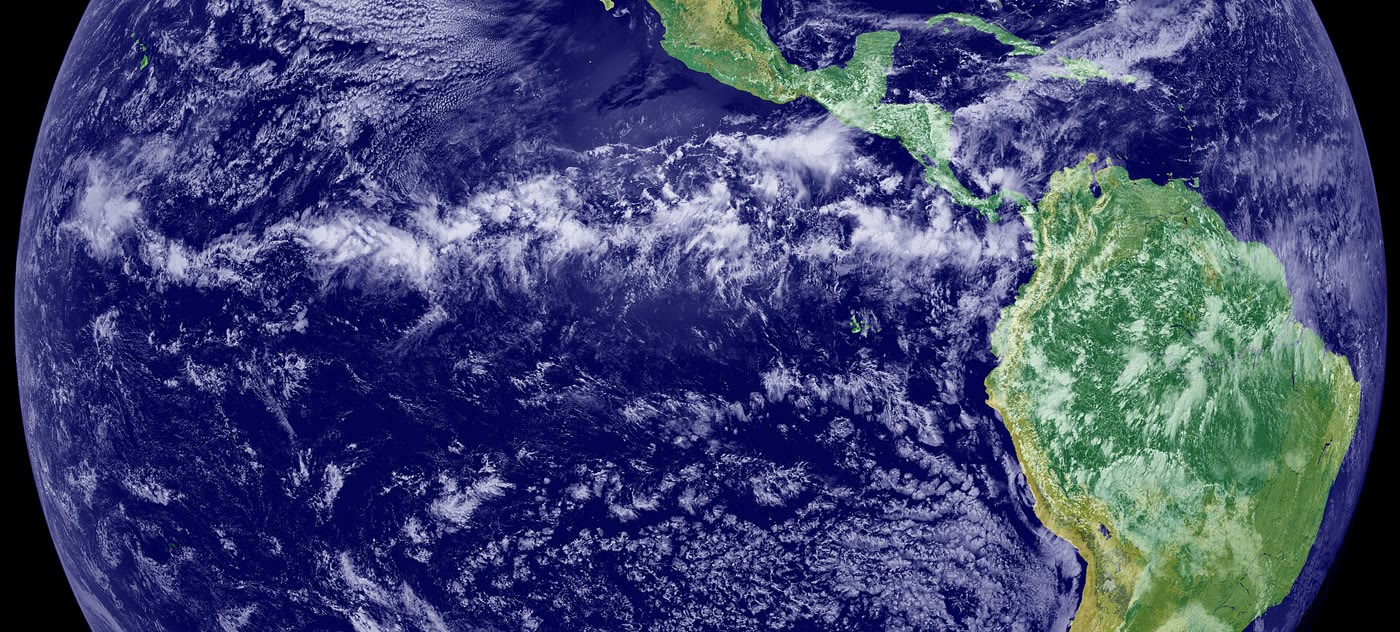
\includegraphics[width=0.8\linewidth]{images/book3/b1-itcz-goes.jpg}

{\small La \omterm{def:b1:atmospheric-circulation:itcz}{zone de convergence intertropicale} sur le Pacifique oriental~: une ligne de
nuages brillants traversant l'océan au nord de l'équateur, avec l'Amérique centrale et
du Sud à droite. L'image combine des données de nuages du satellite géostationnaire
GOES-11 avec des couleurs de la couverture du sol. (NASA Earth Observatory, domaine public, via
Wikimedia Commons.)}
\label{fig:b1:atmospheric-circulation:itcz-photo}
\end{omfigure}
% ledger: commons:itcz-goes

L'air qui converge doit monter, et l'air humide qui monte construit des nuages~: la ZCIT est la ceinture
la plus pluvieuse de la planète, et sa position est repérée par la \omterm{def:b1:spherical-astronomy:geographic}{latitude} où les précipitations
en moyenne zonale culminent. La ZCIT suit le Soleil, avec un retard. Dans la réanalyse le
maximum passe de \ang{12.8}~S en février à \ang{10.9}~N en septembre~; moyennée sur
les douze mois elle se situe à \ang{2.6}~N. La moyenne zonale cache de grandes différences
entre \omterm{def:b1:spherical-astronomy:geographic}{longitudes}~: sur le Pacifique oriental de la photographie la bande se situe au nord
de l'équateur, et une moyenne zonale mêle de telles bandes à d'autres qui oscillent davantage
avec les saisons.
% ledger: data:b3-ncep (computed in figdata/bachelor-1/general_circulation.py)

\begin{omfigure}
\begin{tikzpicture}
\begin{axis}[omrecord, width=0.7\linewidth, height=5.2cm, xmin=0.5, xmax=12.5, ymin=-16, ymax=16,
  xlabel={mois}, ylabel={latitude (\unit{\degree})}, xtick={1,...,12},
  xticklabels={J,F,M,A,M,J,J,A,S,O,N,D}, ytick={-15,-10,...,15}]
% figdata/bachelor-1/general_circulation.py; ledger: data:b3-ncep
\addplot[black!40, domain=0.5:12.5] {0};
\addplot[omThm, line width=1.1pt, mark=*, mark size=1.6pt] table[x=month, y=lat] {figdata/out/bachelor-1-general_circulation-itcz.dat};
\end{axis}
\end{tikzpicture}

{\small La \omterm{def:b1:spherical-astronomy:geographic}{latitude} du maximum de précipitations en moyenne zonale, mois par mois, entre
\ang{20}~S et \ang{20}~N~: la \omterm{def:b1:atmospheric-circulation:itcz}{zone de convergence intertropicale} migre vers le nord dans
l'été boréal et vers le sud dans l'été austral, deux ou trois mois en retard sur le
Soleil.
Réanalyse~1 NCEP-NCAR, moyennes 1991--2020, données fournies par le NOAA PSL.}
\label{fig:b1:atmospheric-circulation:itcz}
\end{omfigure}
% ledger: data:b3-ncep

Le long de l'équateur lui-même, où $f = 0$, l'air se déplace tout droit en descendant le gradient de
pression, et une circulation est--ouest apparaît sur le Pacifique.

\begin{definition}[Circulation de Walker]\label{def:b1:atmospheric-circulation:walker}
La \emph{circulation de Walker}\index{circulation de Walker} est la cellule de retournement est--ouest de
l'atmosphère le long du Pacifique équatorial~: l'air monte sur les eaux chaudes
de l'ouest, autour du Continent maritime, s'écoule vers l'est en altitude, descend sur le Pacifique
oriental et revient vers l'ouest près de la surface avec les \omterm{def:b1:atmospheric-circulation:winds}{alizés}.
\end{definition}
% ledger: climategov:walker

\begin{omfigure}
\begin{tikzpicture}[>={Stealth[length=2mm]}, font=\scriptsize]
  \fill[blue!12] (0,0) rectangle (11,0.45);
  \shade[left color=orange!45, right color=blue!12] (0,0) rectangle (6,0.45);
  \fill[brown!45] (-0.9,0) rectangle (0,0.6);
  \fill[brown!45] (11,0) rectangle (11.9,0.6);
  \node[anchor=north] at (-0.45,-0.05) {Continent};
  \node[anchor=north] at (-0.45,-0.35) {maritime};
  \node[anchor=north] at (11.45,-0.05) {Amérique};
  \node[anchor=north] at (11.45,-0.35) {du Sud};
  \node[anchor=north] at (5.5,-0.05) {océan Pacifique équatorial};
  \node at (1.6,0.22) {eau chaude};
  \foreach \x in {0.6,1.2,1.8} \fill[black!20] (\x,2.6) circle (0.45);
  \foreach \x in {0.9,1.5} \fill[black!25] (\x,3.0) circle (0.4);
  \draw[line width=1.2pt, omThm, ->] (9.5,0.8) -- (2.0,0.8);
  \draw[line width=1.2pt, omThm, ->] (1.2,1.0) -- (1.2,3.0);
  \draw[line width=1.2pt, omThm, ->] (2.0,3.3) -- (9.5,3.3);
  \draw[line width=1.2pt, omThm, ->] (10.3,3.0) -- (10.3,1.0);
  \node[anchor=south] at (5.75,0.85) {alizés, d'est en ouest};
  \node[anchor=south] at (5.75,3.35) {retour en altitude, d'ouest en est};
  \node[anchor=west, align=left] at (1.6,1.8) {air ascendant,\\fortes pluies};
  \node[anchor=east, align=right] at (10.0,1.8) {air subsident,\\sec};
\end{tikzpicture}

{\small La \omterm{def:b1:atmospheric-circulation:walker}{circulation de Walker} le long du Pacifique équatorial (schématique~; hauteur hors
échelle)~: ascendante sur l'ouest chaud, vers l'est en altitude, descendante à l'est et retour
vers l'ouest avec les \omterm{def:b1:atmospheric-circulation:winds}{alizés} près de la surface.}
\label{fig:b1:atmospheric-circulation:walker}
\end{omfigure}
% ledger: climategov:walker

La \omterm{def:b1:atmospheric-circulation:walker}{circulation de Walker} n'est pas stable. Quand elle s'affaiblit, le mouvement ascendant sur le
Continent maritime s'affaiblit et l'air y peut même descendre~; quand elle se renforce,
l'ascendance et la pluie sur l'ouest augmentent. Ces oscillations, El~Niño et La~Niña,
et les renversements saisonniers des moussons sont l'objet du volume de deuxième année.
Sur les décennies depuis 1980, l'évaluation de 2021 du GIEC conclut à un renforcement \emph{très
probable} de la \omterm{def:b1:atmospheric-circulation:walker}{circulation de Walker}, ressemblant à l'état La~Niña, et à un
déplacement vers l'ouest, avec une \emph{confiance moyenne} sur l'ampleur des changements.
% ledger: climategov:walker, ipcc:hadley-widening

\section{Les courants-jets}\label{sec:b1:atmospheric-circulation:jets}

\begin{definition}[Courant-jet~; courants-jets subtropical et du front polaire]\label{def:b1:atmospheric-circulation:jet}
Un \emph{courant-jet}\index{courant-jet} est une étroite bande de vent fort, normalement un
vent horizontal haut dans la troposphère, dont la position change d'un jour à l'autre. Le
\emph{courant-jet subtropical}\index{courant-jet subtropical} souffle de l'ouest près du bord
polaire de la \omterm{def:b1:atmospheric-circulation:cells}{cellule de Hadley}, en général entre \ang{20} et \ang{30} de \omterm{def:b1:spherical-astronomy:geographic}{latitude} à des hauteurs
de \qtyrange{12}{14}{km}. Le \emph{courant-jet du front polaire}\index{courant-jet du front polaire} souffle
de l'ouest au-dessus de la frontière entre l'air polaire et l'air subtropical, entre environ
\ang{50} et \ang{60}~; c'est le noyau rapide des \omterm{def:b1:atmospheric-circulation:winds}{vents d'ouest}, dirigé par les
dépressions et \omterm{def:b1:atmospheric-circulation:cyclone}{anticyclones} des moyennes \omterm{def:b1:spherical-astronomy:geographic}{latitudes} et les dirigeant.
\end{definition}
% ledger: nws:jets, noaajs:jet

Les courants-jets se trouvent typiquement vers \qty{9}{km}, peuvent dépasser
\qty{440}{km/h}, et sont les plus forts dans l'hiver de chaque hémisphère, quand le contraste
de température entre les tropiques et le pôle est le plus grand. Le \omterm{def:b1:atmospheric-circulation:jet}{courant-jet subtropical} est
le vent du moment cinétique de la \cref{prop:b1:atmospheric-circulation:angular-momentum},
apprivoisé par les tourbillons~; il se situe au bord de la \omterm{def:b1:atmospheric-circulation:cells}{cellule de Hadley}, près de \ang{30} dans la
moyenne d'hiver. Le \omterm{def:b1:atmospheric-circulation:jet}{courant-jet du front polaire} oscille vers le nord et le sud avec les
dépressions qui passent, et la moyenne autour du globe l'étale~: dans la moyenne zonale de
l'été boréal il ne reste qu'un faible maximum de \qty{21.6}{m/s} près de \ang{42.5}~N,
et dans l'été austral \qty{29.9}{m/s} près de \ang{47.5}~S. Pourquoi le vent augmente
avec la hauteur partout où la température baisse vers le pôle, le vent thermique, est
montré dans le volume de troisième année.
% ledger: noaajs:jet, nws:jets, data:b3-ncep-circ (computed in figdata/bachelor-1/general_circulation.py)

\section{Exercices}

\begin{exercise}[$\star$]\label{exo:b1:atmospheric-circulation:1}
Prendre $\Omega = \qty{7.292e-5}{rad.s^{-1}}$. (a)~Calculer le \omterm{def:b1:atmospheric-circulation:coriolis-parameter}{paramètre de Coriolis} à
\ang{0}, \ang{30}, \ang{45} et \ang{90}~N. (b)~Calculer l'accélération de Coriolis
horizontale d'un vent de \qty{10}{m/s} à \ang{45}~N et la comparer à $g =
\qty{9.81}{m.s^{-2}}$. (c)~Dans quelle direction pointe-t-elle si le vent souffle
vers le nord~?
% ledger: earth:Trot
\end{exercise}

\begin{exercise}[$\star$]\label{exo:b1:atmospheric-circulation:2}
Deux isobares distantes de \qty{4}{hPa} sont espacées de \qty{400}{km} au niveau de la mer, où $\rho =
\qty{1.225}{kg.m^{-3}}$. (a)~Calculer l'accélération due à la \omterm{def:b1:atmospheric-circulation:pgf}{force de gradient de
pression}. (b)~Si rien d'autre n'agissait, combien de temps faudrait-il pour accélérer l'air immobile jusqu'à
\qty{10}{m/s}~? (c)~Comparer cette accélération à l'accélération de Coriolis d'un vent
de \qty{10}{m/s} à \ang{45}~N, et dire ce que cela suggère.
% ledger: ussa76:sea-level, earth:Trot
\end{exercise}

\begin{exercise}[$\star$]\label{exo:b1:atmospheric-circulation:3}
À \ang{40}~N, des isobares distantes de \qty{4}{hPa} sont espacées de \qty{250}{km}~; prendre $\rho =
\qty{1.225}{kg.m^{-3}}$. (a)~Calculer le \omterm{def:b1:atmospheric-circulation:geostrophic}{vent géostrophique} en \unit{m/s} et en nœuds
(\qty{1}{kn} = \qty{0.5144}{m/s}). (b)~La basse se trouve au sud. D'où
le vent souffle-t-il~? (c)~Décrire la barbule de vent (fût et barbules) qu'un
prévisionniste dessinerait.
% ledger: ussa76:sea-level, earth:Trot
\end{exercise}

\begin{exercise}[$\star$]\label{exo:b1:atmospheric-circulation:4}
Les moyennes annuelles de la réanalyse donnent, près du sol, le vent vers l'est
\qty{-3.5}{m/s} à \ang{15}~N, \qty{-4.4}{m/s} à \ang{15}~S, \qty{+1.9}{m/s} à
\ang{45}~N et \qty{+6.5}{m/s} à \ang{45}~S, et la pression au niveau de la mer
\qty{1011.8}{hPa} à \ang{15}~N, \qty{1016.8}{hPa} à \ang{30}~N et
\qty{1015.8}{hPa} à \ang{45}~N. (a)~Nommer la ceinture de vent à chacune des quatre \omterm{def:b1:spherical-astronomy:geographic}{latitudes}.
(b)~Expliquer le signe de chaque vent avec la branche de surface d'une cellule. (c)~Où est
l'\omterm{def:b1:atmospheric-circulation:cells}{anticyclone subtropical} de l'hémisphère Nord d'après ces pressions~?
% ledger: data:b3-ncep-circ
\end{exercise}

\begin{exercise}[$\star\star$]\label{exo:b1:atmospheric-circulation:5}
Un gradient de pression de \qty{2}{hPa} par \qty{500}{km}, avec $\rho =
\qty{1.225}{kg.m^{-3}}$, est trouvé à \ang{60}, \ang{50}, \ang{30}, \ang{20},
\ang{10} et \ang{5}~N. (a)~Calculer le \omterm{def:b1:atmospheric-circulation:geostrophic}{vent géostrophique} à chaque \omterm{def:b1:spherical-astronomy:geographic}{latitude}.
(b)~Les vents réels des tropiques profonds dépassent rarement quelques mètres par seconde pour de tels
gradients. Expliquer pourquoi l'\omterm{def:b1:atmospheric-circulation:geostrophic}{équilibre géostrophique} échoue près de l'équateur, en utilisant le
temps $1/f$ dont la force de Coriolis a besoin pour tourner le vent.
% ledger: ussa76:sea-level, earth:Trot
\end{exercise}

\begin{exercise}[$\star\star$]\label{exo:b1:atmospheric-circulation:6}
(a)~Avec la \cref{prop:b1:atmospheric-circulation:angular-momentum}, calculer le vent
d'un anneau d'air qui quitte l'équateur au repos, à \ang{10}, \ang{15}, \ang{20} et
\ang{30}~; prendre $\Omega a_\oplus = \qty{464.6}{m/s}$. (b)~La même chose pour un anneau qui
part au repos de \ang{10}, de \ang{15}, de \ang{20} et de \ang{30}. (c)~La branche ascendante
de la \omterm{def:b1:atmospheric-circulation:cells}{cellule de Hadley} est étalée sur des \omterm{def:b1:spherical-astronomy:geographic}{latitudes} plutôt que placée exactement à l'équateur.
Comment cela change-t-il le \omterm{def:b1:atmospheric-circulation:jet}{courant-jet} prévu~?
% ledger: earth:Trot, earth:Rmean
\end{exercise}

\begin{exercise}[$\star\star$]\label{exo:b1:atmospheric-circulation:7}
(a)~Un navire de l'hémisphère Nord a le vent du sud-ouest. En utilisant la loi de Buys
Ballot, où est le centre de basse pression~? (b)~Un navire de l'hémisphère
Sud a le vent du nord-ouest. Où est la basse~? (c)~Près du sol le
vent coupe les isobares vers les basses pressions. Cela change-t-il votre réponse à (a)
en tournant la direction de la basse dans le sens horaire ou trigonométrique~?
% ledger: skybrary:buys-ballot
\end{exercise}

\begin{exercise}[$\star\star$]\label{exo:b1:atmospheric-circulation:8}
(a)~Calculer la masse d'air comprise entre l'équateur et \ang{30}~N et entre les
niveaux de pression \qty{1000}{hPa} et \qty{100}{hPa}, avec $a_\oplus = \qty{6371}{km}$
et $g = \qty{9.81}{m.s^{-2}}$. (b)~En moyenne annuelle la \omterm{def:b1:atmospheric-circulation:cells}{cellule de Hadley} nord de la
réanalyse porte \qty{8.7e10}{kg/s}. Combien de temps faudrait-il pour faire passer cette masse
une fois à travers la cellule~? (c)~Même question avec la cellule de l'hiver boréal,
\qty{21.4e10}{kg/s}.
% ledger: earth:Rmean, data:b3-ncep-circ
\end{exercise}

\begin{exercise}[$\star\star$]\label{exo:b1:atmospheric-circulation:9}
Supposons que sous un \omterm{def:b1:atmospheric-circulation:cells}{anticyclone subtropical} l'air descende à \qty{1}{cm/s}, et qu'il soit
non saturé. (a)~De quelle distance descend-il en un jour~? (b)~De combien se réchauffe-t-il en un jour,
si rien d'autre n'agit, avec le \omterm{def:b1:fluid-envelopes-structure:lapse-rate}{gradient adiabatique sec} de \qty{9.8}{K/km}~? (c)~
L'air ne se réchauffe pas autant jour après jour. Quel processus du
\cref{ch:b1:radiation-heat-transport} compense le réchauffement~? (d)~Pourquoi beaucoup des
grands déserts chauds se trouvent-ils sous ces \omterm{def:b1:atmospheric-circulation:cyclone}{anticyclones}~?
% ledger: nws:dalr
\end{exercise}

\begin{exercise}[$\star\star\star$]\label{exo:b1:atmospheric-circulation:10}
À \ang{50}~N, prendre $f = \qty{1.117e-4}{s^{-1}}$ et des isobares circulaires de rayon
$r = \qty{500}{km}$ (\cref{rem:b1:atmospheric-circulation:gradient}). (a)~Autour d'une
basse où le \omterm{def:b1:atmospheric-circulation:geostrophic}{vent géostrophique} serait de \qty{15}{m/s}, résoudre $V^2/r + fV =
f|\vec v_g|$ pour le vent de gradient $V$. (b)~Autour d'une haute, montrer que $V^2/r - fV + f
|\vec v_g| = 0$ n'a de solution que si $|\vec v_g| \leq fr/4$, et calculer cette limite.
(c)~Qu'implique (b) pour l'espacement des isobares près du centre d'un
\omterm{def:b1:atmospheric-circulation:cyclone}{anticyclone}, comparé à une dépression~?
\end{exercise}

\begin{exercise}[$\star\star\star$]\label{exo:b1:atmospheric-circulation:11}
(a)~Montrer que pour de petits $\varphi$ (en radians) le vent d'un anneau quittant l'équateur
au repos est $u \approx \Omega a_\oplus\varphi^2$. (b)~Comparer l'approximation à
la formule exacte à \ang{10}, avec $\Omega a_\oplus = \qty{464.6}{m/s}$. (c)~Le
vent annuel moyen de la réanalyse à \qty{200}{hPa} culmine à \qty{27.0}{m/s} près de
\ang{35}~N. À quelle \omterm{def:b1:spherical-astronomy:geographic}{latitude} l'anneau atteindrait-il cette vitesse~? (d)~Que dit la
réponse de la mesure dans laquelle l'argument du moment cinétique peut être cru~?
% ledger: earth:Trot, earth:Rmean, data:b3-ncep-circ
\end{exercise}

\begin{exercise}[$\star\star\star$]\label{exo:b1:atmospheric-circulation:12}
Les précipitations en moyenne zonale de la réanalyse culminent aux \omterm{def:b1:spherical-astronomy:geographic}{latitudes} suivantes, de
janvier à décembre~: \ang{-10.5}, \ang{-12.8}, \ang{-5.8}, \ang{-4.6}, \ang{5.5},
\ang{7.3}, \ang{8.6}, \ang{10.4}, \ang{10.9}, \ang{9.1}, \ang{7.4}, \ang{6.2}
(négatif~: sud). (a)~Calculer la moyenne annuelle et l'étendue. (b)~La \omterm{def:b1:spherical-astronomy:geographic}{latitude} subsolaire
est extrême en juin et en décembre. De combien de mois la ZCIT est-elle en retard
sur elle, et qu'est-ce qui, dans le système climatique, peut stocker de la chaleur et causer un tel retard~?
(c)~Supposons que sur un océan la ZCIT reste au nord de l'équateur toute l'année. Expliquer
comment la moyenne zonale peut tout de même traverser l'équateur.
% ledger: data:b3-ncep
\end{exercise}

\section{Problème~: Lire une carte météorologique de moyennes latitudes}

\begin{problem}[{Problème du week-end --- le vent à une station près de \ang{50}~N}]
\label{pb:b1:atmospheric-circulation:1}
% values: calc/ch28.py (invented map; jet from data:b3-ncep-circ)
Une carte météorologique de l'Atlantique Nord montre, près d'une station P à \ang{50}~N, des
isobares rectilignes allant d'ouest en est, tous les \qty{4}{hPa}, avec les pressions plus basses
au nord. P se trouve entre les isobares \qty{1004}{hPa} et \qty{1008}{hPa}, qui sont
espacées de \qty{250}{km} en ce lieu~; sa pression au niveau de la mer est de \qty{1006}{hPa} et la
température de l'air de \qty{10}{\degreeCelsius}. La carte est inventée, mais ses nombres sont typiques.
Utiliser $\Omega = 2\pi/(\qty{23.9345}{h})$, $a_\oplus = \qty{6371}{km}$, $R_d =
\qty{287.05}{J.kg^{-1}.K^{-1}}$ pour l'air sec, \qty{1}{kn} = \qty{0.514444}{m/s}.

\medskip
\noindent\textbf{Partie I --- Le gradient de pression et le vent géostrophique.}
\begin{enumerate}
  \item Calculer la masse volumique de l'air en P avec la loi des gaz parfaits.
  \item Calculer le gradient horizontal de pression en P, en \unit{Pa.m^{-1}}.
  \item Calculer l'accélération due à la \omterm{def:b1:atmospheric-circulation:pgf}{force de gradient de pression}.
  \item Calculer $\Omega$ et le \omterm{def:b1:atmospheric-circulation:coriolis-parameter}{paramètre de Coriolis} à \ang{50}~N.
  \item Calculer la vitesse du \omterm{def:b1:atmospheric-circulation:geostrophic}{vent géostrophique} en P.
  \item L'exprimer en nœuds et en \unit{km/h}.
  \item Montrer que le temps dont la seule \omterm{def:b1:atmospheric-circulation:pgf}{force de gradient de pression} aurait besoin pour amener
        de l'air immobile à la vitesse géostrophique est $1/f$, et le calculer, avec
        le temps $2\pi/f$ que la force de Coriolis met à faire tourner un vent d'un tour complet.
\end{enumerate}

\medskip
\noindent\textbf{Partie II --- Direction et hémisphère.}
\begin{enumerate}[resume]
  \item Dans quelle direction pointe la \omterm{def:b1:atmospheric-circulation:pgf}{force de gradient de pression} en P~? Dans quelle
        direction souffle le \omterm{def:b1:atmospheric-circulation:geostrophic}{vent géostrophique}, et de quel \omterm{def:b1:spherical-astronomy:horizontal}{azimut}
        vient-il~?
  \item Vérifier votre réponse avec la loi de Buys Ballot.
  \item Décrire la barbule de vent dessinée en P~: la direction du fût, le nombre
        de barbules, et le côté où elles se placent.
  \item Supposons que les mêmes isobares, avec la basse au nord, se trouvent à
        \ang{50}~S. D'où le vent soufflerait-il~?
  \item Avec la même masse volumique et le même gradient de pression, calculer le \omterm{def:b1:atmospheric-circulation:geostrophic}{vent géostrophique}
        à \ang{30}~N et \ang{60}~N.
  \item Le calculer à \ang{5}~N. Le résultat est-il crédible~? Expliquer.
\end{enumerate}

\medskip
\noindent\textbf{Partie III --- Le vent au sol.} Un anémomètre en P mesure un
vent de \qty{9.0}{m/s} coupant les isobares à \ang{25} vers les basses pressions.
\begin{enumerate}[resume]
  \item Calculer le rapport du vent observé au \omterm{def:b1:atmospheric-circulation:geostrophic}{vent géostrophique}, et les
        composantes du vent observé le long des isobares et à travers elles.
  \item De quel \omterm{def:b1:spherical-astronomy:horizontal}{azimut} le vent observé souffle-t-il~?
  \item Dans le modèle de traînée linéaire de la \cref{prop:b1:atmospheric-circulation:friction},
        quelle constante de temps $\tau$ donne l'angle observé, et quelle vitesse le
        modèle prédit-il alors~? Comparer avec l'observation.
  \item Autour d'une dépression de rayon \qty{500}{km}, supposons que l'air du
        premier kilomètre s'écoule vers l'intérieur partout avec la composante transversale aux isobares
        de la question~14 et la masse volumique de la question~1. Calculer la masse d'air
        entrant dans la dépression par seconde.
  \item Cet air doit sortir par le haut de la couche. Calculer la vitesse ascendante moyenne
        en ce lieu, en \unit{m/s} et en mètres par jour.
  \item Au \omterm{def:b1:fluid-envelopes-structure:lapse-rate}{gradient adiabatique sec} de \qty{9.8}{K/km}, de combien l'air
        ascendant se refroidit-il en un jour~? Quel temps s'ensuit-il, et que se passerait-il
        sous un \omterm{def:b1:atmospheric-circulation:cyclone}{anticyclone} à la place~?
\end{enumerate}

\medskip
\noindent\textbf{Partie IV --- Le courant-jet au-dessus.} Le vent en moyenne zonale à \qty{200}{hPa} dans
l'hiver boréal culmine à \qty{42.3}{m/s} près de \ang{30}~N (moyennes de réanalyse
1991--2020).
\begin{enumerate}[resume]
  \item Calculer la vitesse vers l'est du sol à l'équateur et à \ang{30}~N.
  \item Un anneau d'air quitte l'équateur au repos en altitude et garde son moment
        cinétique. Calculer son vent à \ang{20}~N et \ang{30}~N.
  \item Même question à \ang{30}~N pour un anneau qui part au repos de \ang{10}~N.
  \item De quel facteur l'anneau de la question~21 dépasse-t-il le \omterm{def:b1:atmospheric-circulation:jet}{courant-jet} observé à
        \ang{30}~N~? Donner deux raisons pour lesquelles le \omterm{def:b1:atmospheric-circulation:jet}{courant-jet} réel est plus lent.
  \item Calculer le rapport du moment cinétique absolu par unité de masse du
        \omterm{def:b1:atmospheric-circulation:jet}{courant-jet} observé à \ang{30}~N à celui de l'air au repos à l'équateur. Quelle
        fraction a été perdue en chemin~?
  \item Quelle est la vitesse du \omterm{def:b1:atmospheric-circulation:geostrophic}{vent géostrophique} en P, en mètres par seconde, et comment
        le vent mesuré au sol se compare-t-il à elle~?
\end{enumerate}
\end{problem}
